\documentclass{beamer}
\usepackage[utf8]{inputenc}

\usepackage{semantic}
\usepackage{graphicx}
\usepackage{booktabs}
%\usepackage{todonotes}
\usepackage[absolute,overlay]{textpos}
\usepackage{tikz}

\mode<presentation> {
\usetheme{boxes} % When headline is wanted use Dresden theme instead
\usecolortheme{seagull}
\setbeamertemplate{footline}[page number]
\setbeamertemplate{navigation symbols}{}
}


% APL LaTeX declarations, based on work by A.Hohti/O.Kanerva
% University of Helsinki April 6 1987
%
% Written Oct. 3rd 2006 by Markus Triska (triska@gmx.at)
% Public domain code.

\font\apl=cmapl10 at 9pt      % The APL font of typewriter type

% from:
%		apldef.tex
%
% 2-letter control sequences for using cmapl10.
%===============================================================
%
\def\RO{{\apl\char'014}}               % rho
\def\IO{{\apl\char'015}}               % iota
\def\BX{\hskip0pt\lower.1ex\hbox{\apl\char'001}}               % quad box (window etc.)
\def\CE{{\apl\char'035}}               % ceiling
\def\FL{{\apl\char'034}}               % floor
\def\DE{{\apl\char'031}}               % decode
\def\EN{{\apl\char'030}}               % encode
\def\DL{{\apl\char'002}}               % del
\def\LD{{\apl\char'003}}               % delta
\def\NT{{\apl\char'026}}               % not
\def\LO{{\apl\char'017}}               % circle
\def\GO{{\apl\char'036}}               % arrow right
\def\OR{{\apl\char'010}}               % logical or
\def\DM{{\apl\char'011}}               % diamond
\def\LE{{\apl\char'012}}               % less than or equal
\def\GE{{\apl\char'013}}               % greater than or equal
\def\AB{{\apl\char'174}}               % stile
\def\LB{{\apl\char'173}}               % left brace
\def\RB{{\apl\char'175}}               % right brace
\def\DA{{\apl\char'037}}               % arrow down
\def\UA{{\apl\char'136}}               % arrow up
\def\EP{{\apl\char'006}}               % epsilon
\def\NE{{\apl\char'027}}               % not equal
\def\BL{{\apl\char'134}}               % backslash
\def\RU{{\apl\char'022}}               % right U
\def\LU{{\apl\char'023}}               % left U
\def\DU{{\apl\char'021}}               % down U
\def\UU{{\apl\char'020}}               % up U
\def\LK{{\apl\char'033}}               % right tack
\def\RK{{\apl\char'032}}               % left tack
\def\US{{\apl\char'024}}               % underscore
\def\NG{{\apl\char'025}}               % high minus
\def\DD{{\apl\char'007}}               % dieresis
\def\AM{{\apl\char'004}}               % alpha
\def\OM{{\apl\char'005}}               % omega
\def\SO{\leavevmode\raise.3ex\hbox{{\apl\char'016}}} % small circle
%
% This macro is used for overstriking two characters
\newskip\charwidth
\def\overstrike#1#2{\setbox1=\hbox{#1}\charwidth=\wd1
           #1\hskip-\charwidth#2}
%
\def\TR{\overstrike{\LO}{\BL}}                              % transpose
\def\RV{\overstrike{\LO}{\AB}}                              % reverse
\def\CR{\overstrike{\leavevmode\raise.1ex\hbox{\hskip0.361pt -}}{\LO}}
                                                   % column reverse
\def\GD{\overstrike{\DL}{\AB}}                              % grade down
\def\GU{\overstrike{\LD}{\AB}}                              % grade up
\def\FM{\overstrike{\leavevmode\raise.1ex\hbox{{\apl\char'016}}}{\EN}} % format
\def\XQ{\overstrike{\leavevmode\raise.1ex\hbox{{\apl\char'016}}}{\DE}} % execute
\def\SS{\overstrike{\RU}{\US}}                              % subset
\def\CO{\overstrike{\LU}{\US}}                              % contains
\def\CB{\overstrike{\BL}{-}}                                % column backslash
\def\CS{\overstrike{/}{-}}                                  % column slash
\def\IB{\overstrike{\EN}{\DE}}                              % I-beam
\def\DQ{\overstrike{{\apl\char'045}}{\BX}}                  % divide quad
\def\QQ{\overstrike{{\apl '}}{\BX}}                         % quote quad
\def\PD{\overstrike{\DL}{\NT}}                              % protected del
\def\NR{\overstrike{\OR}{\NT}}                              % nor
\def\NN{\overstrike{{\apl\char'046}}{\NT}}                  % nand
\def\LG{\overstrike{{\apl *}}{\LO}}                         % logarithm
\def\PO{\overstrike{\DD}{\apl *}}
% underscored letters
\def\ZA{\overstrike{{\apl A}}{\US}}
\def\ZB{\overstrike{{\apl B}}{\US}}
\def\ZC{\overstrike{{\apl C}}{\US}}
\def\ZD{\overstrike{{\apl D}}{\US}}
\def\ZE{\overstrike{{\apl E}}{\US}}
\def\ZF{\overstrike{{\apl F}}{\US}}
\def\ZG{\overstrike{{\apl G}}{\US}}
\def\ZH{\overstrike{{\apl H}}{\US}}
\def\ZI{\overstrike{{\apl I}}{\US}}
\def\ZJ{\overstrike{{\apl J}}{\US}}
\def\ZK{\overstrike{{\apl K}}{\US}}
\def\ZL{\overstrike{{\apl L}}{\US}}
\def\ZM{\overstrike{{\apl M}}{\US}}
\def\ZN{\overstrike{{\apl N}}{\US}}
\def\ZO{\overstrike{{\apl O}}{\US}}
\def\ZP{\overstrike{{\apl P}}{\US}}
\def\ZQ{\overstrike{{\apl Q}}{\US}}
\def\ZR{\overstrike{{\apl R}}{\US}}
\def\ZS{\overstrike{{\apl S}}{\US}}
\def\ZT{\overstrike{{\apl T}}{\US}}
\def\ZU{\overstrike{{\apl U}}{\US}}
\def\ZV{\overstrike{{\apl V}}{\US}}
\def\ZX{\overstrike{{\apl X}}{\US}}
\def\ZY{\overstrike{{\apl Y}}{\US}}
\def\ZW{\overstrike{{\apl W}}{\US}}
\def\ZZ{\overstrike{{\apl Z}}{\US}}

% unicode declarations

% first row
\DeclareUnicodeCharacter{22C4}{\DM} % diamond
\DeclareUnicodeCharacter{223C}{\NT} % not
\DeclareUnicodeCharacter{00A8}{\DD} % dieresis
\DeclareUnicodeCharacter{2336}{\IB} % I-Beam
\DeclareUnicodeCharacter{00AF}{\NG} % high minus
\DeclareUnicodeCharacter{236B}{\PD} % protected del
\DeclareUnicodeCharacter{2352}{\GD} % grade down
\DeclareUnicodeCharacter{2264}{\LE} % less than or equal
\DeclareUnicodeCharacter{234B}{\GU} % grade up
\DeclareUnicodeCharacter{233D}{\RV} % reverse
\DeclareUnicodeCharacter{2265}{\GE} % greater or equal
\DeclareUnicodeCharacter{2349}{\TR} % transpose
\DeclareUnicodeCharacter{2296}{\CR} % column reverse
\DeclareUnicodeCharacter{2260}{\NE} % not equal
\DeclareUnicodeCharacter{235F}{\LG} % logarithm
\DeclareUnicodeCharacter{2228}{\OR} % logical or
\DeclareUnicodeCharacter{2371}{\NR} % nor
\DeclareUnicodeCharacter{2227}{{\apl\char'046}} % and
\DeclareUnicodeCharacter{2372}{\NN} % nand
\DeclareUnicodeCharacter{00D7}{{\apl\char'043}} % times
\DeclareUnicodeCharacter{00F7}{{\apl\char'045}} % division
\DeclareUnicodeCharacter{2339}{\DQ} % divide quad / matrix division
% second row
\DeclareUnicodeCharacter{2375}{\OM} % omega
\DeclareUnicodeCharacter{2208}{\EP} % epsilon
\DeclareUnicodeCharacter{2377}{\overstrike{\EP}{\US}} % underscore epsilon
\DeclareUnicodeCharacter{2374}{\RO} % rho
\DeclareUnicodeCharacter{2191}{\UA} % up arrow
\DeclareUnicodeCharacter{2193}{\DA} % down arrow
\DeclareUnicodeCharacter{2373}{\IO} % iota
\DeclareUnicodeCharacter{2378}{\overstrike{\IO}{\US}} % underscore iota
\DeclareUnicodeCharacter{25CB}{\LO} % circle
\DeclareUnicodeCharacter{2365}{\overstrike{\DD}{\LO}} % circle dieresis
\DeclareUnicodeCharacter{22C6}{{\apl *}} % exponentiation
\DeclareUnicodeCharacter{235F}{\LG} % logarithm
\DeclareUnicodeCharacter{2190}{{\apl\char'137}} % arrow left
\DeclareUnicodeCharacter{2192}{\GO} % arrow right
\DeclareUnicodeCharacter{2340}{\CB} % column backslash
\DeclareUnicodeCharacter{2359}{\overstrike{\US}{\LD}} % delta underscore
% third row
\DeclareUnicodeCharacter{237A}{\AM} % alpha
\DeclareUnicodeCharacter{2296}{\CR} % column reverse
\DeclareUnicodeCharacter{2308}{\CE} % ceiling
\DeclareUnicodeCharacter{230A}{\FL} % floor
\DeclareUnicodeCharacter{2261}{$\equiv$}
\DeclareUnicodeCharacter{2207}{$\nabla$}
\DeclareUnicodeCharacter{2352}{\GD} % grade down
\DeclareUnicodeCharacter{2206}{\LD} % delta
\DeclareUnicodeCharacter{2218}{\SO} % jot
\DeclareUnicodeCharacter{2364}{\"\relax\hskip-5.8pt\SO} % jot dieresis
\DeclareUnicodeCharacter{233C}{\overstrike{\BX}{\LO}} % quad circle
\DeclareUnicodeCharacter{2395}{\BX} % quad
\DeclareUnicodeCharacter{235E}{\QQ} % quote quad
\DeclareUnicodeCharacter{22A2}{\LK} % right tack
\DeclareUnicodeCharacter{2342}{\overstrike{\BX}{\BL}} % quad backslash
\DeclareUnicodeCharacter{22A3}{\RK} % left tack
\DeclareUnicodeCharacter{233C}{\overstrike{\BX}{\LO}} % quad circle
\DeclareUnicodeCharacter{2282}{\RU} % right u
\DeclareUnicodeCharacter{2283}{\LU} % left u
\DeclareUnicodeCharacter{2229}{\DU} % down u
\DeclareUnicodeCharacter{235D}{{\apl\char'042}} % comment sign
\DeclareUnicodeCharacter{222A}{\UU} % up u
\DeclareUnicodeCharacter{22A5}{\DE} % decode
\DeclareUnicodeCharacter{234E}{\XQ} % execute
\DeclareUnicodeCharacter{22A4}{\EN} % encode
\DeclareUnicodeCharacter{2355}{\FM} % format
\DeclareUnicodeCharacter{2223}{\AB} % stile
\DeclareUnicodeCharacter{233F}{\CS} % column slash
\DeclareUnicodeCharacter{2212}{-}   % minus
\DeclareUnicodeCharacter{2262}{$\not\equiv$}
\DeclareUnicodeCharacter{220A}{\EP} % small contains, alternative for member
\DeclareUnicodeCharacter{2217}{{\apl *}} % asterisk, alternative for star
\DeclareUnicodeCharacter{03BA}{$\kappa$}
\DeclareUnicodeCharacter{2363}{\overstrike{\DD}{{\apl *}}}

\newcommand{\kw}[1]{\texttt{#1}}
\newcommand{\A}[2]{[#1]^{#2}}
\newcommand{\V}[2]{\langle#1\rangle^{#2}}
\renewcommand{\S}[2]{\textrm{S}_{#1}(#2)}
\newcommand{\SV}[2]{\textrm{SV}_{#1}(#2)}
\newcommand{\id}[1]{\textit{#1}}

\newcommand{\IOt}{\texttt{\IO}}
\newcommand{\DDt}{\texttt{\DD}}
\newcommand{\ROt}{\texttt{\RO}}
\newcommand{\UAt}{\texttt{\UA}}
\newcommand{\DAt}{\texttt{\DA}}
\newcommand{\LUt}{\texttt{\LU}}
\newcommand{\TRt}{\texttt{\TR}}
\newcommand{\RVt}{\texttt{\RV}}
\newcommand{\POt}{\texttt{\PO}}
\newcommand{\FMt}{\texttt{\FM}}


%----------------------------------------------------------------------------------------
%	TITLE PAGE
%----------------------------------------------------------------------------------------

\title[APL \& TAIL] % bottom of every slide
  {Compiling a subset of APL to a \\ Typed Array Intermediate Language} % title page

\author{\footnotesize{Martin Dybdal} \\ \footnotesize{\texttt{dybber@dybber.dk}}}

\institute {
HIPERFIT \\
DIKU \\
University of Copenhagen
}

\date{\footnotesize{Chalmers, 10 October 2015}}

% \title[Group Theory]{A longer title of the talk concerning Group Theory}
% \author[short name]{My full name}
% \institute[My Inst.]{Full Institut Name}
% % logo of my university

\date[10 October 2015]{10 October 2015 \\ \vspace{1cm} \footnotesize{Joint work with Martin Elsman and Michael Budde}}

\begin{document}

{
\setbeamertemplate{headline}{}
\begin{frame}
\titlepage
\end{frame}
}

%----------------------------------------------------------------------------------------
%	TABLE OF CONTENTS
%----------------------------------------------------------------------------------------

% \begin{frame}
% \frametitle{Overview}
% \tableofcontents
% \end{frame}

%----------------------------------------------------------------------------------------
%	CONTENT
%----------------------------------------------------------------------------------------


\section{Overview}

\begin{frame}
\frametitle{Goals}
\begin{itemize}
\item GPU programming for APL fingers
\item Develop backend technology independently of APL. Other frontends
  could be J, K, some new Haskell vector-library or R-library.
\item Bridging the PL and APL communities
  % \begin{itemize}
  % \item APL compiler writers have been doing fusion since 1970 (at
  %   least), originally they called it ``drag-along''.
  % \end{itemize}
\item Performance on code written by non-programmers (e.g. biologist
  or quant code)
\end{itemize}

\end{frame}


\begin{frame}
\frametitle{Why APL?}
\begin{itemize}
\item 
Notation for non-programmers (biologist/chemist/quants etc.)
\item 
APLs primitives have proven suitable for many applications
\item 
\textbf{APL programs are inherently parallel}
  \begin{quotation}
    \noindent
    "Unlike other languages, the problem in APL is not determining
    where parallelism exists. Rather, it is to decide what to do with
    all of it." \\
      - Robert Bernecky, 1993
  \end{quotation}
\item Existing programs/benchmarks (this is not such a strong point as
  we originally thought)
% \begin{itemize}
% \item We don't have to write our own
% \item Writing the benchmarks ourselves might not represent how it will
%   be used in a production environment
% %\item Writing our own is not always trustworthy. We can specialise
% %  them towards the compiler.
% %\item We want to perform on biologist- and quant-written code.
% \end{itemize}
\end{itemize}

\end{frame}

\begin{frame}
\frametitle{Overview}

\begin{itemize}
\item APL: Dynamically weakly typed array language
\item TAIL: Statically strongly typed array language as target for APL
  and friends.
  \begin{itemize}
  \item type inference
  \item polymorphic shape-types (similar to Repa/Accelerate shapes)
  \item singleton-types
  \item no nested arrays
  \item no heterogeneous arrays
  \end{itemize}
\end{itemize}

\end{frame}

\begin{frame}
\frametitle{Restrictions}
\begin{itemize}
\item No nested arrays or nested parallelism
\item Lexical scoping (ISO APL Standard specifies dynamic scoping)
\item No efficient implementation of boolean arrays as bit-arrays
\item No dynamic conversions between integer and doubles (APL normally
  does this e.g. if overflow would otherwise occur)
\item Reshapes not possible when size of shape-vector is unknown
\item Several built-ins are still missing
\item No labels and gotos, only limited branching
\item No recursion
\end{itemize}
\end{frame}

\begin{frame}[fragile]
\frametitle{Brief APL introduction}


\begin{verbatim}
⍳5
    1 2 3 4 5

⍴⍳5
    5

2⍴⍳5
    1 2

2 4⍴⍳5
    1 2 3 4
    5 1 2 3

⍴2 4⍴⍳5
    2 4
\end{verbatim}

\end{frame}

\begin{frame}[fragile]
\frametitle{Brief APL introduction}

Function definitions:
\begin{verbatim}
    add ← {⍺ × 100 + ⍵}
    10 add 42
        1420
\end{verbatim}

Implicit vectorisation:
\begin{verbatim}
    7 9 13 = 3 9 15
        0 1 0
\end{verbatim}

\pause
Equality of all elements can be written:
\begin{verbatim}
    7 9 13 {∧/,⍺=⍵} 3 9 15
        0

    7 9 13 {∧/,⍺=⍵} 7 9 13
        1
\end{verbatim}
(or you can use the built in match-operator: \verb|≡|)

\begin{textblock*}{40mm}(0.70\textwidth,0.40\textheight)
\only<3->{
\begin{block}{Try it yourself}
\url{http://tryapl.org/}
\end{block}
}
\end{textblock*}

\end{frame}

\begin{frame}[fragile]
\frametitle{Brief APL introduction}

\begin{verbatim}
    ⍳5
        1 2 3 4 5
\end{verbatim}

\begin{verbatim}
    (1 10 100)∘.+(⍳5)
          2   3   4   5   6
         11  12  13  14  15
        101 102 103 104 105
\end{verbatim}

\pause
Upper triangular matrix idiom:
\begin{verbatim}
    (⍳5)∘.≤(⍳5)
        1 1 1 1 1
        0 1 1 1 1
        0 0 1 1 1
        0 0 0 1 1
        0 0 0 0 1
\end{verbatim}


\pause
Idioms library: \url{http://aplwiki.com/FinnAplIdiomLibrary}

\end{frame}

\section{TAIL}

\begin{frame}
\frametitle{TAIL}

  \begin{itemize}
  \item \textbf{Make vectorisation and scalar extensions explicit}
  \item \textbf{Statically determine array ranks and shapes (when possible)}
  \item Insert numeric coercions
  \item Resolve overloading of numeric operations
  \item Resolve % identity items (for reductions) and
    default arguments
    (e.g. for over takes)
  \item Resolve overloading of shape operations
  \end{itemize}

\end{frame}


\begin{frame}[fragile]
\frametitle{Example: APL $->$ TAIL}
{\footnotesize
\begin{verbatim}
pi ← { 
 x ← ?⍵⍴0
 y ← ?⍵⍴0
 dists ← (x*2) + y*2
 4×(+/1>dists)÷⍵
}
pi 1000000
    3.142668
\end{verbatim}
\pause
\vspace{-2mm}
$\quad\Downarrow$
\vspace{-2mm}
% muld(4.0,
%  divd(i2d(
%    reduce(addi,0,
%      each(b2i,
%        each(fn v7:[double]0 => gtd(1.0,v7),
%          each(fn v6:[double]0 => powd(v6,divd(1.0,2.0)),
%            reduce(addd,0.0,
%              each(fn v3:[double]0 => powd(v3,2.0),
%                each(fn v2:[bool]0 => roll(b2i(v2)),
%                     reshape([1000000,2],[ff]))))))))),
%       1000000.0))
\begin{verbatim}
let v3:[double]1 = 
  each(fn v2:[int]0 => roll(v2), reshape([1000000],[0])) in
let v5:[double]1 =
  each(fn v4:[int]0 => roll(v4), reshape([1000000],[0])) in
let v11:[double]1 = 
  each(fn v10:[double]0 => powd(v10,divd(1.0,2.0)),
       zipWith(addd, each(fn v7:[double]0 => powd(v7,2.0),v3),
                     each(fn v6:[double]0 => powd(v6,2.0),v5))) in
muld(4.0, divd(i2d(reduce(addi,0,
                     each(b2i,
                       each(fn v12:[double]0 => gtd(1.0,v12),
                            v11)))),
               1000000.0))
\end{verbatim}
}

\begin{textblock*}{64mm}(0.50\textwidth,0.43\textheight)
\only<2->{
\begin{block}{\vspace*{-3ex}}
Note: \texttt{each} is just \texttt{map} in APL lingo
\end{block}
}
\end{textblock*}

\end{frame}



% \begin{frame}[fragile]
% \frametitle{Parallelism opportunities in APL programs}

% \begin{itemize}
% \item Implicit maps for arguments ranks higher than function rank, for example reduction of a 2D array (SIMD)
%   \begin{verbatim}
%   pi ← { 4×(+/1>(+/(?⍵ 2⍴0)*2)*÷2)÷⍵ }
%   \end{verbatim}
% \item Built in parallelisable functions: reduce, scan, joins, etc. (SIMD)
% \item Expression-level and inter-line parallelism (MIMD)
% \end{itemize}
% \end{frame}


\begin{frame}[fragile]
\frametitle{Implicit vectorisation}

\textit{Most} APL primitives are defined for a specific argument rank
$k$, but in the case it is applied to any array with a rank higher
than $k$ it will be applied \textit{independently} to each rank-k
subarray.

\begin{block}{Negation}
\vspace{-4mm}
\begin{verbatim}-17
    ¯17

-⍳6
    ¯1 ¯2 ¯3 ¯4 ¯5 ¯6

-2 3⍴⍳6
    ¯1 ¯2 ¯3
    ¯4 ¯5 ¯6
\end{verbatim}
\vspace{-4mm}
\end{block}
\end{frame}

\begin{frame}[fragile]
\frametitle{Implicit vectorisation}

In TAIL we make vectorisation explicit by inserting
applications of \texttt{each} and \texttt{zipWith}:\\

$$\texttt{each} : \forall\alpha\beta\gamma.~(\alpha -> \beta) ->
  [\alpha]^\gamma -> [\beta]^{\gamma}$$
$$\texttt{zipWith} :
  \forall\alpha_1\alpha_2\beta\gamma.~(\alpha_1 -> \alpha_2 -> \beta)
  -> [\alpha_1]^\gamma -> [\alpha_2]^\gamma -> [\beta]^{\gamma}$$


\begin{block}{Example}
\vspace{-4mm}
\begin{verbatim}
(2 3⍴1) + (2 3⍴⍳6)
\end{verbatim}

$\quad\Downarrow$

\begin{verbatim}
zipWith(addi, reshape([2,3], [1]),
              reshape([2,3], iota(6)))
\end{verbatim}
\vspace{-4mm}
\end{block}
\end{frame}


\begin{frame}[fragile]
\frametitle{Implicit vectorisation}

In some cases, applying ``\kw{each}'' is not what we want:

\begin{block}{Reduction}
\vspace{-4mm}
\begin{verbatim}
+/1 2 3 4
    10

2 3⍴⍳6
    1 2 3
    4 5 6

+/2 3⍴⍳6   ⍝ sum each row
    6 15
\end{verbatim}
\vspace{-4mm}
\end{block}


\end{frame}

\begin{frame}[fragile]
\frametitle{Implicit vectorisation}

Instead we make reductions work directly on arrays with $rank > 0$ (like Accelerate).

$$\texttt{reduce} : \forall\alpha\gamma. (\alpha -> \alpha -> \alpha) -> \alpha -> [\alpha]^{1+\gamma} -> [\alpha]^{\gamma}$$

\begin{block}{Reduction translation}
\vspace{-4mm}
\begin{verbatim}
+/2 3⍴⍳6   ⍝ sum each row
\end{verbatim}
$\quad\Downarrow$

\begin{verbatim}
reduce(addi, reshape([2,3], iota(6)))
\end{verbatim}
\vspace{-4mm}
\end{block}

It still holds that: \textit{Most APL primitives are defined for a
  specific argument rank $k$, but in the case it is applied to any
  array with a rank higher than $k$ it will be applied
  \textit{independently} to each rank-k subarray.}
\end{frame}

\begin{frame}[fragile]
\frametitle{Built-ins}

{\tiny
$$
\begin{array}{llcl}
  \id{APL} & \id{op}(s) & & {\rm TySc}(\id{op}) \\ \hline
    &\kw{addi},\ldots & : & \kw{int} -> \kw{int} -> \kw{int} \\
    &\kw{addd},\ldots & : & \kw{double} -> \kw{double} -> \kw{double} \\
  \IOt & \kw{iota} & : & \kw{int} -> \A{\kw{int}}{1} \\
  \DDt &\kw{each} & : & \forall \alpha \beta \gamma. (\alpha -> \beta) -> \A{\alpha}{\gamma} -> \A{\beta}{\gamma} \\
    &\kw{zipWith} & : & \forall \alpha_1\alpha_2 \beta \gamma. ({\alpha_1} -> {\alpha_2} -> \beta) -> \A{\alpha_1}{\gamma} -> \A{\alpha_2}{\gamma} -> \A{\beta}{\gamma} \\
  \kw{/} &\kw{reduce} & : & \forall \alpha \gamma. (\alpha -> \alpha -> \alpha) -> \alpha  -> \A{\alpha}{1+\gamma} -> \A{\alpha}{\gamma} \\
  \kw{/} &\kw{compress} & : & \forall \alpha \gamma. \A{\kw{bool}}{\gamma} -> \A{\alpha}{\gamma} -> \A{\alpha}{\gamma} \\
  \kw{/} &\kw{replicate} & : & \forall \alpha \gamma. \A{\kw{int}}{\gamma} -> \A{\alpha}{\gamma} -> \A{\alpha}{\gamma} \\
  \verb+\+ & \kw{scan} & : & \forall \alpha \gamma. (\alpha -> \alpha -> \alpha) -> \A{\alpha}{\gamma} -> \A{\alpha}{\gamma} \\
  \ROt &\kw{shape} & : & \forall \alpha \gamma. \A{\alpha}{\gamma} -> \V{\kw{int}}{\gamma} \\
  % \ROt &\kw{reshape0} & : & \forall \alpha \gamma \gamma'. \V{\kw{int}}{\gamma'} -> \A{\alpha}{\gamma} -> \A{\alpha}{\gamma'} \\
  \ROt &\kw{reshape} & : & \forall \alpha \gamma \gamma'. \V{\kw{int}}{\gamma'} -> \alpha -> \A{\alpha}{\gamma} -> \A{\alpha}{\gamma'} \\
  \RVt &\kw{reverse} & : & \forall \alpha \gamma. \A{\alpha}{\gamma} -> \A{\alpha}{\gamma} \\
  \RVt &\kw{rotate} & : & \forall \alpha \gamma. \kw{int} -> \A{\alpha}{\gamma} -> \A{\alpha}{\gamma} \\
  \TRt &\kw{transp} & : & \forall \alpha \gamma. \A{\alpha}{\gamma} -> \A{\alpha}{\gamma} \\
  \TRt &\kw{transp2} & : & \forall \alpha \gamma. \V{\kw{int}}{\gamma} -> \A{\alpha}{\gamma} -> \A{\alpha}{\gamma} \\
  \UAt &\kw{take} & : & \forall \alpha \gamma. \kw{int} -> \alpha -> \A{\alpha}{\gamma} -> \A{\alpha}{\gamma} \\
  \DAt &\kw{drop} & : & \forall \alpha \gamma. \kw{int} -> \A{\alpha}{\gamma} -> \A{\alpha}{\gamma} \\
  % \LUt &\kw{first} & : & \forall \alpha \gamma. \alpha -> \A{\alpha}{\gamma} -> \alpha \\
  , &\kw{cat} & : & \forall \alpha \gamma. \A{\alpha}{\gamma+1} -> \A{\alpha}{\gamma+1} -> \A{\alpha}{\gamma+1} \\
  , &\kw{cons} & : & \forall \alpha \gamma. \A{\alpha}{\gamma} -> \A{\alpha}{\gamma+1} -> \A{\alpha}{\gamma+1} \\
  , &\kw{snoc} & : & \forall \alpha \gamma. \A{\alpha}{\gamma+1} -> \A{\alpha}{\gamma} -> \A{\alpha}{\gamma+1} \\
  % \FMt & \kw{formatI} & : & \kw{int} -> \A{\kw{char}}{1} \\
  % \FMt & \kw{formatD} & : & \kw{double} -> \A{\kw{char}}{1}
\end{array}
$$
}

\textit{(incomplete list)}
\end{frame}


\begin{frame}[fragile]
\frametitle{Shape types}

We need to know the length of the shape-vector, to be able to infer
the rank of the resulting array of a reshape!

$$
\begin{array}{llcl}
  \id{APL} & \id{op}(s) & & {\rm TySc}(\id{op}) \\ \hline
  \ROt &\kw{shape} & : & \forall \alpha \gamma. \A{\alpha}{\gamma} -> \V{\kw{int}}{\gamma} \\
  % \ROt &\kw{reshape0} & : & \forall \alpha \gamma \gamma'. \V{\kw{int}}{\gamma'} -> \A{\alpha}{\gamma} -> \A{\alpha}{\gamma'} \\
  \ROt &\kw{reshape} & : & \forall \alpha \gamma \gamma'. \V{\kw{int}}{\gamma'} -> \alpha -> \A{\alpha}{\gamma} -> \A{\alpha}{\gamma'} \\
  % \TRt &\kw{transp2} & : & \forall \alpha \gamma. \V{\kw{int}}{\gamma} -> \A{\alpha}{\gamma} -> \A{\alpha}{\gamma} \\
\end{array}
$$

  \begin{itemize}
  \item $\V{\kw{int}}{\gamma}$ is a length $\gamma$ integer vector
  \item $\A{\alpha}{\gamma}$ is an array with rank $\gamma$
  \end{itemize}

  \vspace{4mm} \textit{Limitation wrt. APL: We must know the length of
    the shape-vector statically, e.g. it cannot be the result of a
    filter.}

\end{frame}

% \begin{frame}[fragile]
%   \frametitle{Shape types} 
%   When reshaping an array and the length of the shape-vector is
%   statically known, we will always know the rank of the resulting
%   array.

%   $$\kw{reshape} : \forall\alpha\gamma\gamma'. \V{\kw{int}}{\gamma'} -> \alpha -> \A{\alpha}{\gamma} -> \A{\alpha}{\gamma'}$$

%   \begin{itemize}
%   \item $\V{\kw{int}}{\gamma'}$ is a length $\gamma'$ integer vector
%   \item $\A{\alpha}{\gamma'}$ is an array with rank $\gamma'$
%   \end{itemize}

%   \vspace{4mm} \textit{Limitation wrt. APL: We must know the length of
%     the shape-vector statically, e.g. it cannot be the result of a
%     filter.}

% \end{frame}

\begin{frame}[fragile]
\frametitle{Type system}

\begin{align*}
\kappa & ::= \kw{int} ~~|~~ \kw{double} ~~|~~ \kw{bool} ~~|~~ \kw{char} ~~|~~ \alpha \tag{base types} \\
\rho & ::= i ~~|~~ \gamma ~~|~~ \rho + \rho' \tag{shape types} \\
\tau & ::= \A{\kappa}{\rho} ~~|~~ \V{\kappa}{\rho} ~~|~~ \S{\kappa}{\rho} ~~|~~ \SV{\kappa}{\rho} \\
 &  ~~|~~ \tau -> \tau' \tag{types} \\
\sigma & ::= \forall \vec{\alpha} \vec{\gamma}.\tau \tag{type schemes}
\end{align*}

\begin{itemize}
\item Shape types are tree structured to support \texttt{drop} and
  \texttt{catenate} on vectors (unlike Accelerate)
\item $\S{\kw{int}}{\rho}$ is the singleton integer $\rho$ (rank-0)
\item $\SV{\kw{int}}{\rho}$ is a singleton integer vector with element $\rho$  (rank-1)
\item We often write $\kappa$ instead of $[\kappa]^0$
\end{itemize}
\end{frame}

\begin{frame}[fragile]
\frametitle{Shape operations}

We need to be able to calculate on shapes, retaining
length-information.

$$
\begin{array}{llcl}
  \id{APL} & \id{op}(s) & & {\rm TySc}(\id{op}) \\ \hline
  \ROt &\kw{shapeV}  & : & \forall\alpha\gamma. \V{\alpha}{\gamma} -> \SV{\kw{int}}{\gamma} \\
  \UAt &\kw{takeV}   & : & \forall\alpha\gamma. \S{\kw{int}}{\gamma} -> \A{\alpha}{1} -> \V{\alpha}{\gamma} \\
  \DAt &\kw{dropV}   & : & \forall\alpha\gamma\gamma'. \S{\kw{int}}{\gamma} -> \V{\alpha}{(\gamma+\gamma')} -> \V{\alpha}{\gamma'} \\
  % ,    &\kw{consV}   & : & \forall\alpha\gamma. \alpha -> \V{\alpha}{\gamma} -> \V{\alpha}{(1+\gamma)} \\
  % ,    &\kw{snocV}   & : & \forall\alpha\gamma. \V{\alpha}{\gamma} -> \alpha -> \V{\alpha}{(1+\gamma)} \\
  % \LUt &\kw{firstV}  & : & \forall\alpha\gamma. \SV{\alpha}{\gamma} -> \S{\alpha}{\gamma} \\
  \IOt &\kw{iotaV}   & : & \forall \gamma. \S{\kw{int}}{\gamma} -> \V{\kw{int}}{\gamma} \\
  \RVt &\kw{rotateV} & : & \forall\alpha\gamma. \V{\alpha}{\gamma} -> \V{\alpha}{\gamma} \\
  ,    &\kw{catV}    & : & \forall\alpha\gamma\gamma'. \V{\alpha}{\gamma} -> \V{\alpha}{\gamma'} -> \V{\alpha}{(\gamma + \gamma')}
\end{array}
$$

\textit{(incomplete list)}

\end{frame}

\begin{frame}[fragile]
\frametitle{Subtyping rules}

We might know the vector sizes or integer values statically, but want
to use them where that information is not needed:

\begin{verbatim}
  let v0:<int>100 = iotaV(100) in
  reduce(addi,0,v0)
\end{verbatim}

To make the singleton integers and vectors with known length
compatible with functions taking general arrays, we add subtyping:

\begin{equation*}
\frac{}{\tau \subseteq \tau}\hspace{1cm}
\frac{\tau_1 \subseteq \tau_2 ~~~ \tau_2 \subseteq \tau_3}{\tau_1 \subseteq \tau_3}
\end{equation*}

\begin{equation*}
\frac{}{\V{\kappa}{\rho} \subseteq \A{\kappa}{1}}\hspace{1cm}
\frac{}{\S{\kappa}{\rho} \subseteq \A{\kappa}{0}}\hspace{1cm}
\frac{}{\SV{\kappa}{\rho} \subseteq \V{\kappa}{1}}
\end{equation*}

%We use a type inference algorithm based on conditional unification.

\end{frame}

\begin{frame}[fragile]
\frametitle{Example: APL $->$ TAIL}

% TODO: find better example, including reshape operation and computed
% shapes in Accelerate-output.

\begin{verbatim}
diff ← {1↓⍵−¯1⌽⍵}
signal ← {¯50⌈50⌊50×(diff 0,⍵)÷0.01+⍵}
+/ signal ⍳ 100
\end{verbatim}

\pause
$\quad\Downarrow$

\footnotesize
\begin{verbatim}
let v0:<int>100 = iotaV(100) in
let v3:<int>101 = consV(0,v0) in
reduce(addd,0.00,
 each(fn v11:[double]0 => maxd(~50.00,v11),
  each(fn v10:[double]0 => mind(50.00,v10),
   each(fn v9:[double]0 => muld(50.00,v9),
    zipWith(divd,
     each(i2d,
       drop(1,zipWith(subi,v3,rotateV(~1,v3)))),
     eachV(fn v2:[double]0 => addd(0.01,v2),
       eachV(i2d,v0)))))))
\end{verbatim}
\end{frame}

\begin{frame}[fragile]
\frametitle{APL $->$ TAIL $->$ ?}
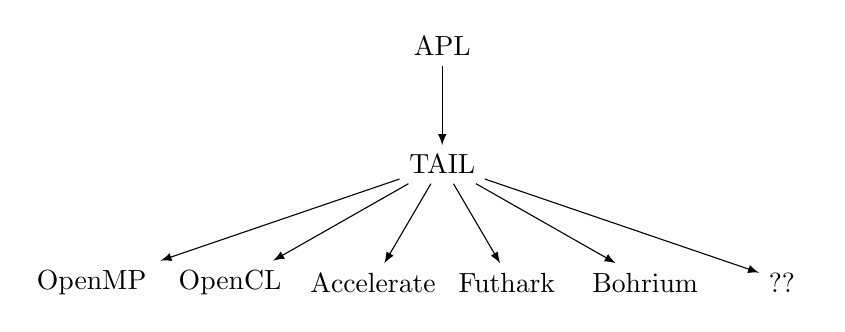
\begin{tikzpicture}[edge from parent/.style={draw,-latex},
                    sibling distance=5em,
                    every node/.style = {shape=rectangle,
                    align=center}]
  \node {APL}
    child { node {TAIL}
      child { node { OpenMP } } 
      child { node { OpenCL } } 
      child { node {Accelerate} }
      child { node { Futhark } } 
      child { node { Bohrium } } 
      child { node { ?? } } 
    };
\end{tikzpicture}

\end{frame}

\begin{frame}[fragile]
\frametitle{Why targeting Accelerate? }

\begin{itemize}
\item Seemed like an obvious choice given the similarities with TAIL
\item The Accelerate people had shown interest
\item Using their segmented reductions and scans, we could potentially
  also perform NESL-like flattening and thus allow nested computations.
\end{itemize}

A lot of hurdles came up, mostly because the EDSL-nature of
Accelerate. More on that later!
\end{frame}

\begin{frame}[fragile]
\frametitle{Example: TAIL $->$ Accelerate}

\tiny
\begin{verbatim}
module Main where
import qualified Prelude as P
import Prelude ((+), (-), (*), (/))
import Data.Array.Accelerate
import qualified Data.Array.Accelerate.CUDA as Backend
import qualified APLAcc.Primitives as Prim
 
program :: Acc (Scalar P.Double)
program
  = let v0 = Prim.iotaV 100 :: Acc (Array DIM1 P.Int) in
      let v3
            = Prim.consV (constant (0 :: P.Int)) v0 :: Acc (Array DIM1 P.Int)
        in
        Prim.reduce (+) (constant (0.0 :: P.Double))
          (Prim.each (\ v11 -> P.max (constant (-50.0 :: P.Double)) v11)
             (Prim.each (\ v10 -> P.min (constant (50.0 :: P.Double)) v10)
                (Prim.each (\ v9 -> constant (50.0 :: P.Double) * v9)
                   (Prim.zipWith (/)
                      (Prim.each Prim.i2d
                         (Prim.drop (constant (1 :: P.Int))
                            (Prim.zipWith (-) v3
                               (Prim.transp
                                  (Prim.rotateV (constant (-1 :: P.Int)) (Prim.transp v3))))))
                      (Prim.eachV (\ v2 -> constant (1.0e-2 :: P.Double) + v2)
                         (Prim.eachV Prim.i2d v0))))))
main = P.print (Backend.run program)
\end{verbatim}

\end{frame}

\begin{frame}
\frametitle{Benchmarks}

\begin{tabular}{llrr}
\textbf{Benchmark} & \textbf{Problem size} & \textbf{TAIL C} & \textbf{TAIL Acc} \\
\midrule
Integral       & N = 10,000,000 &  46.90 &    3.10 \\
Signal         & N = 50,000,000 & 209.03 &   16.1  \\
Game-of-Life   & $40\times 40$, N = 2,000 &  28.70 & 2.30 \\
Easter         & N = 3,000 &   33.96 &         -  \\
Black-Scholes  & N = 10,000&    54.0 &      -     \\
Sobol MC $\pi$ & N = 10,000,000  & 4881.30  &   2430.30   \\
HotSpot        & $1024\times 1024$, N = 360 &    6072.93 &   2.03
\end{tabular}

\vspace{1cm}

\begin{itemize}
\item Timings in milliseconds. Averages over 30 executions.
\end{itemize}

\end{frame}


\begin{frame}
\frametitle{Difficulties using Accelerate}

(I might be too honest here!)

\begin{itemize}
\item No easy to target AST-representation (yet) and generating
  Haskell code is not ideal
\item Shapes in Accelerate have the outer-most dimension placed
  innermost in the the Shape-list. Making certain operations difficult
  to implement efficiently (e.g. vertical rotation)
\item When using Accelerate looping constructs (e.g. \texttt{awhile})
  it seems that sharing is not recovered (e.g. let bound variables
  outside the loop are inlined, into the loop)
\item No real cost-model. We are unable to reason about memory layout
  (e.g. after a transposition).
\item No control over memory allocations
\item Hard to debug
\item Hard to benchmark% . You have to use various tricks to force a
  % computation, and avoid including time spent by calling \texttt{nvcc}.
\item No mutable array updates
\end{itemize}

\end{frame}

\begin{frame}
\frametitle{What I'm working on while at Chalmers}

~APL \\
$\quad\Downarrow$ \\
~TAIL $\quad\Rightarrow\quad$Accelerate \\
$\quad\Downarrow$\\
~~\ldots \\
$\quad\Downarrow$ \\
~~\ldots \\
$\quad\Downarrow$ \\
\fbox{Some new functional low-level GPU intermediate language} \\
$\quad\Downarrow$ \\
OpenCL/CUDA
\end{frame}

%------------------------------------------------

\begin{frame}
\frametitle{Requirements}
\begin{itemize}
% \item Interpreted environment (e.g. APL, MATLAB, NumPy, R)
%   \begin{itemize}
%   \item implies dynamic compilation (JIT)
%   \item implies dynamic garbage collection
%   \end{itemize}

\item Ability to optimise
  \begin{itemize}
  \item Consistent cost-model
  \item Control over memory allocations
  \item Control over when fusion/materialization occurs
  \end{itemize}
\item (Array updates in sequential code of kernel bodies)

% \item Optimised idioms (e.g. 100x100 identity matrix: (⍳100)∘.=(⍳100),
%   should be represented as a sparse matrix)
\end{itemize}
\end{frame}

% \begin{frame}
%   \frametitle{Next steps}
%   \begin{itemize}
%   \item Frontend
%     \begin{itemize}
%     \item Add array indexing
%     \item Support DNA-application from Dyalog
%     \item Support benchmarks from various old APL-papers
%     \end{itemize}
%   \item Accelerate backend
%     \begin{itemize}
%     \item Convert TAIL shapes to Accelerate shapes correctly
%     \item Type-checker targetting their HOAS representation
%     \item Mersenne Twister in Accelerate
%     \item Support more primitives
%     \end{itemize}
%   \end{itemize}
% \end{frame}

\defverbatim{\tc}{%
\begin{verbatim}
equal ← { ∧/,⍺=⍵ }

pi ← { 4×(+/1>+/(?⍵ 2⍴0)*2)÷⍵ }

tc ← { ({⍵∨⍵∨.∧⍵} ⍣ ≡) ⍵ }
\end{verbatim}
}

\defverbatim{\tcanno}{%
\begin{verbatim}
⍝○ equal : [a]r → [a]r → bool
equal ← { ∧/,⍺=⍵ }

⍝○ pi : int → double
pi ← { 4×(+/1>(+/(?⍵ 2⍴0)*2)*÷2)÷⍵ }

⍝○ [bool]2 → [bool]2
tc ← { ({⍵∨⍵∨.∧⍵} ⍣ ≡) ⍵ }
\end{verbatim}
}

\begin{frame}[fragile]
  \frametitle{Latest addition: Type annotations in APL code}

\only<1>{\tc}
\only<2->{\tcanno
Disclosure: still pretty buggy}

\end{frame}

\begin{frame}[fragile]
  \frametitle{Benefits of type annotations}

  \begin{itemize}
  \item Easier debugging, through improved error messages
  \item Machine checked documentation
  \item A necessity for compiling certain programs - even
    parsing APL is undecidable!
  \item Will allow for introducing dependent types, with user-written
    types. (e.g. tracking complete shape information, not just ranks)
  \item First steps towards a module system for APL, supporting
    separate compilation of modules.
  \end{itemize}

\end{frame}

\begin{frame}
  \frametitle{Other future work on TAIL}
  \begin{itemize}
  \item Annotations for GPU vs. CPU execution
  \item Other annotations controlling code generation (not clear what
    they should be yet)
  \item Ability to drop down to a lower level (like inline assembler)
  \item Tracking complete shape information, using dependent types
    (like QUBE)
  \item Region-inference for memory management
  \item Additional primitives
  \item Integration with real APL interpreter (Dyalog)
  % \item JIT compilation
  % \item Support nested arrays (flattening or through SNESL?)
  % \item Boolean array encode/decode?
  \end{itemize}
\end{frame}

\begin{frame}
\frametitle{References}
\footnotesize{
\begin{thebibliography}{99} % Beamer does not support BibTeX so references must be inserted manually as below
\bibitem{p1} Compiling a Subset of APL Into a Typed Intermediate Language.
\newblock Martin Elsman and Martin Dybdal, 2014
\newblock \emph{ARRAY'14}

\bibitem{p1} Compiling APL to Accelerate through a Typed Array Intermediate Language
\newblock Michael Budde, Martin Dybdal and Martin Elsman, 2014
\newblock \emph{ARRAY'15}

\bibitem{p1} Accelerating Haskell array codes with multicore GPUs
\newblock MMT Chakravarty, G Keller, S Lee, TL McDonell, V Grover, 2011
\newblock \emph{DAMP'11}

\bibitem{p1} APEX: The APL Parallel Executor
\newblock Robert Bernecky, 1997
\newblock \emph{Master Thesis}

\bibitem{p1} QUBE - Array Programming with Dependent Types
\newblock Kai Trojahner, 2011
\newblock \emph{Ph.D. thesis}

\end{thebibliography}
}
\end{frame}

\begin{frame}
\Huge{\centerline{Questions?}}
\end{frame}


%----------------------------------------------------------------------------------------
%	BEAMER EXAMPLES of column layouts and tables
%----------------------------------------------------------------------------------------

% \begin{frame}
% \frametitle{Multiple Columns}
% \begin{columns}[c] % The "c" option specifies centered vertical alignment while the "t" option is used for top vertical alignment

% \column{.45\textwidth} % Left column and width

% \column{.5\textwidth} % Right column and width

% \end{columns}
% \end{frame}

% \begin{frame}
% \frametitle{Table}
% \begin{table}
% \begin{tabular}{l l l}
% \toprule
% \textbf{Treatments} & \textbf{Response 1} & \textbf{Response 2}\\
% \midrule
% Treatment 1 & 0.0003262 & 0.562 \\
% Treatment 2 & 0.0015681 & 0.910 \\
% Treatment 3 & 0.0009271 & 0.296 \\
% \bottomrule
% \end{tabular}
% \caption{Table caption}
% \end{table}
% \end{frame}

\end{document}